\documentclass[a4paper,11pt]{article}
\usepackage{amsmath,amsthm,amsfonts,amssymb,amscd,amstext,vmargin,graphics,graphicx,tabularx,multicol} \usepackage[french]{babel}
\usepackage[utf8]{inputenc}  
\usepackage[T1]{fontenc} 
\usepackage[T1]{fontenc}
\usepackage{amsmath,amssymb}
\usepackage{pstricks-add,tikz,tkz-tab,variations}
\usepackage[autolanguage,np]{numprint} 

\setmarginsrb{1.5cm}{0.5cm}{1cm}{0.5cm}{0cm}{0cm}{0cm}{0cm} %Gauche, haut, droite, haut
\newcounter{numexo}
\newcommand{\exo}[1]{\stepcounter{numexo}\noindent{\bf Exercice~\thenumexo} : \marginpar{\hfill /#1}}
\reversemarginpar


\newcounter{enumtabi}
\newcounter{enumtaba}
\newcommand{\q}{\stepcounter{enumtabi} \theenumtabi.  }
\newcommand{\qa}{\stepcounter{enumtaba} (\alph{enumtaba}) }
\newcommand{\initq}{\setcounter{enumtabi}{0}}
\newcommand{\initqa}{\setcounter{enumtaba}{0}}

\newcommand{\be}{\begin{enumerate}}
\newcommand{\ee}{\end{enumerate}}
\newcommand{\bi}{\begin{itemize}}
\newcommand{\ei}{\end{itemize}}
\newcommand{\bp}{\begin{pspicture*}}
\newcommand{\ep}{\end{pspicture*}}
\newcommand{\bt}{\begin{tabular}}
\newcommand{\et}{\end{tabular}}
\renewcommand{\tabularxcolumn}[1]{>{\centering}m{#1}} %(colonne m{} centrée, au lieu de p par défault) 
\newcommand{\tnl}{\tabularnewline}

\newcommand{\trait}{\noindent \rule{\linewidth}{0.2mm}}
\newcommand{\hs}[1]{\hspace{#1}}
\newcommand{\vs}[1]{\vspace{#1}}

\newcommand{\N}{\mathbb{N}}
\newcommand{\Z}{\mathbb{Z}}
\newcommand{\R}{\mathbb{R}}
\newcommand{\C}{\mathbb{C}}
\newcommand{\Dcal}{\mathcal{D}}
\newcommand{\Ccal}{\mathcal{C}}
\newcommand{\mc}{\mathcal}

\newcommand{\vect}[1]{\overrightarrow{#1}}
\newcommand{\ds}{\displaystyle}
\newcommand{\eq}{\quad \Leftrightarrow \quad}
\newcommand{\vecti}{\vec{\imath}}
\newcommand{\vectj}{\vec{\jmath}}
\newcommand{\Oij}{(O;\vec{\imath}, \vec{\jmath})}
\newcommand{\OIJ}{(O;I,J)}

\newcommand{\bmul}[1]{\begin{multicols}{#1}}
\newcommand{\emul}{\end{multicols}}


\newcommand{\reponse}[1][1]{%
\multido{}{#1}{\makebox[\linewidth]{\rule[0pt]{0pt}{20pt}\dotfill}
}}

\newcommand{\titre}[5] 
% #1: titre #2: haut gauche #3: bas gauche #4: haut droite #5: bas droite
{
\noindent #2 \hfill #4 \\
#3 \hfill #5

\vspace{-1.6cm}

\begin{center}\rule{6cm}{0.5mm}\end{center}
\vspace{0.2cm}
\begin{center}{\large{\textbf{#1}}}\end{center}
\begin{center}\rule{6cm}{0.5mm}\end{center}
}



\begin{document}
\pagestyle{empty}
\titre{Contrôle : Angles et nombres relatifs}{Nom :}{Prénom :}{Classe}{Date}


\exo{4}

\bmul{3}
$T= (-0,7) + (-1,8)$

\columnbreak
$V= +10 - (-32) - (+7) + (-9)$

\columnbreak
$I= - 7,5 - (18 - 7,3) - (2 - 14,5)$
\emul

\noindent \q Simplifier l'écriture des expressions T et V.\\
\q Calculer les expressions T, V et I.\\

\exo{2}
Pour chacune des questions suivantes, le calcul doit être écrit.\\

\noindent \initq \q L'empire de Césarius a été créé en – 330 et s'est terminé en 213. Combien de temps a-t-il duré ?\\
\q Antonionus est né en – 211. Il a vécu 63 ans. En quelle année est-il mort ?\\


\exo{1,5} Un négociant achète une moto 1 800 euros, puis il la revend aussitôt 2 500 euros. Il achète aussi une voiture 3 300 euros qu'il revend 2 900 euros.\\

\initq 
\noindent \q Écrire une expression B qui traduit le bilan de ces achats et de ces ventes.\\
\q Calculer B et interpréter le résultat.\\



\exo{3}

\initq 
\noindent \q Placer sur une droite graduée les points A, B et C d'abscisses respectives 2,3 ; -3,7 et -0,7.\\
\q Calculer les distances AC et BC.\\
\q Que peut-on dire du point C ? (Justifier)\\

\exo{1,5} Dans chaque brique, le nombre à inscrire est la somme des deux nombres situés en dessous. Compléter les cases vides: \\

\begin{center}
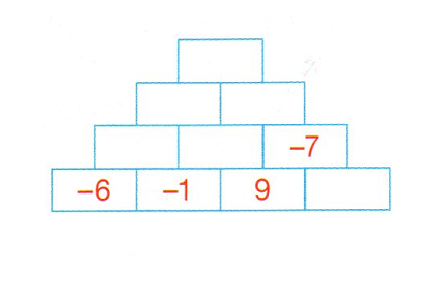
\includegraphics[scale=1]{pyramide.eps} 
\end{center}



\exo{2,5} QCM \\

\bmul{2}
A l'aide de la figure ci-contre, répondre aux questions du
tableau.\\
Pour chaque question, mettre la lettre correspondant à la
bonne réponse dans la dernière case.

\columnbreak

\includegraphics[scale=1]{angles1.eps} 

\emul


\includegraphics[scale=1]{qcm.eps} \\


\exo{1,5}

\bmul{2}

\begin{flushleft}
\includegraphics[scale=1]{dtespara.eps} 
\end{flushleft}

\columnbreak

\textbf{Démontrer} que les droites (d') et (d'') sont parallèles.

\emul

\exo{4}

\begin{center}
\includegraphics[scale=1]{axodur.eps} \\

\end{center}
\initq 
\q On donne $\widehat{NBA}$= 105 degré. Quelle est la mesure de l'angle $\widehat{ABT}$ ?\\
\q \textbf{Démontrer} que l'angle $\widehat{XAB}$ mesure 105 degré.\\
\q Et quelle est la mesure de l'angle $\widehat{YAM}$ ? (Justifier votre réponse à l'aide d'une \textbf{démonstration})\\

\exo{} BONUS\\

Compléter ce carré magique de façon que les sommes des nombres écrits sur une même ligne, sur une même colonne ou sur une même diagonale soient égales.\\

\begin{center}
\includegraphics[scale=1]{carremag.eps} 
\end{center}






\end{document}
